
%----------------------------------------------------------------------------------------
%	Lecture 1
%----------------------------------------------------------------------------------------

\section*{\centering Derivatives, Slope, Velocity \ Rate of Change}  

\bigbreak
\section{Geometric Viewpoint on Derivatives}

\begin{figure}[h!]
	\centering
	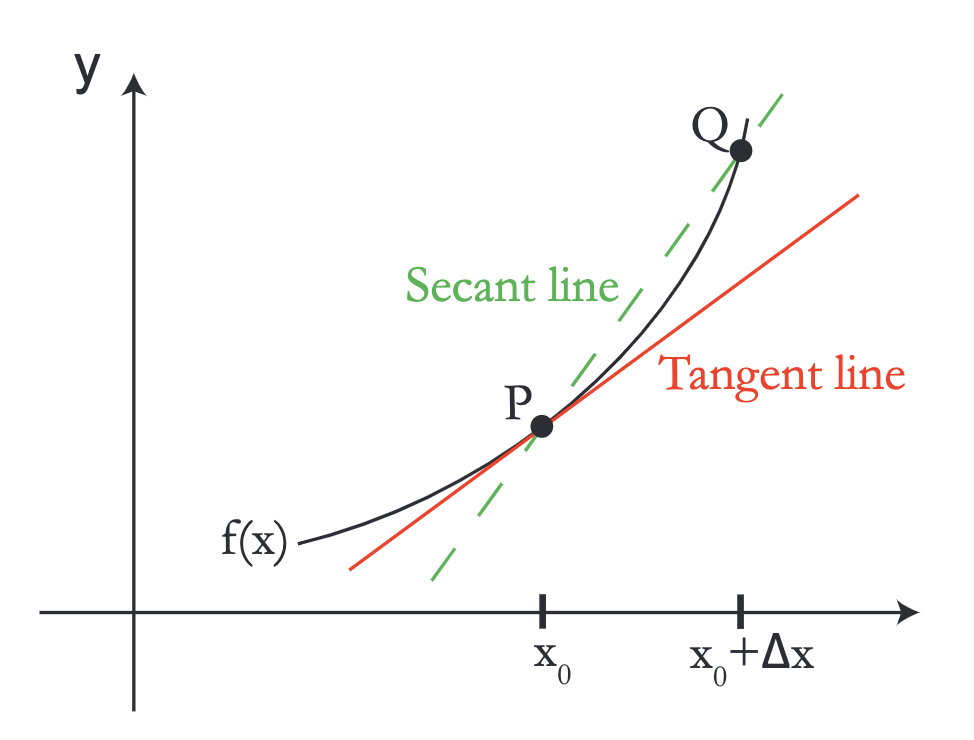
\includegraphics[scale=0.3]{./images/lecture_1_figure_1.png}
	\caption{A function with secant and tangent lines}
\end{figure}

The derivative is the slope of the line tangent to the graph of f(x).
The tangent line is the limit of the secant line as the distance between the two points goes to zero.

\subsection{Geometric Definition of the derivative}

\begin{figure}[h]
	\centering
	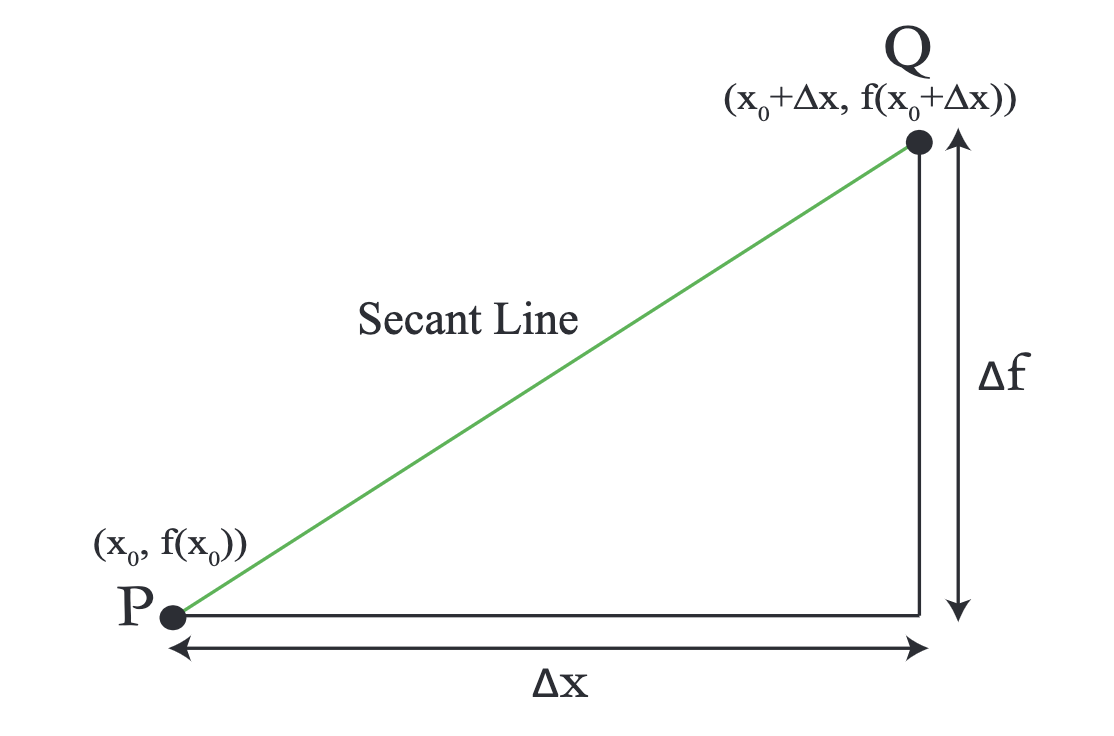
\includegraphics[scale=0.5]{./images/lecture_1_figure_2.png}
	\caption{Geometric definition of a derivative}
\end{figure}

\begin{equation*}
	\lim_{\Delta x \to 0} \frac{\Delta f}{\Delta x} 
	= \lim_{\Delta x \to 0} \underbrace{\frac{f(x+\Delta x) - f(x)}{\Delta x}}_\text{``difference quotient''} = f'(x)
\end{equation*}


It is NOT just a line that meets the graph at one point. 
It is the limit of the secant line (a line drawn between two points on the graph) as the distance between the two points goes to zero.
